\documentclass[11pt,pdftex,twoside,a4paper]{article}
\usepackage{amsthm}
\usepackage{array}
\usepackage{dsfont}
\usepackage{enumitem}
\usepackage{graphicx}
\usepackage{relsize}
\usepackage{float}

\input{mymacs}

% Undefine the conflicting commands
\let\dddot\undefined
\let\ddddot\undefined
\usepackage{accents}
\usepackage{centernot}


\newcommand{\AC}{\ensuremath{\mathop{\rm AC}\nolimits}}
\newcommand{\B}[1]{\textbf{#1}}
\newcommand{\Cohen}{\mathop{\rm Cohen}\nolimits}
\newcommand{\MA}{\ensuremath{\mathop{\rm MA}\nolimits}}
\newcommand{\ccc}{c.c.c.}
\newcommand{\CH}{\ensuremath{\mathop{\rm CH}\nolimits}}
\newcommand{\cof}{\ensuremath{\mathop{\rm cof}\nolimits}}
\newcommand{\Col}{\ensuremath{\mathop{\rm Col}\nolimits}}
\newcommand{\crotin}{\rotatebox[origin=c]{-90}{\(\in\)}}
\newcommand{\dsP}{\ensuremath{\mathds{P}}}
\newcommand{\finitepartial}{\textnormal{finite partial}}
\newcommand{\forces}{\ensuremath{\Vdash}}
\newcommand{\forcesstar}{\ensuremath{\Vdash^*}}
\newcommand{\GCH}{\ensuremath{\mathop{\rm GCH}\nolimits}}
\newcommand{\Lev}{\ensuremath{\mathop{\rm Lev}\nolimits}}
\newcommand{\kcc}{\(\kappa\).c.c}
\newcommand{\MG}{\ensuremath{M[G]}}
\newcommand{\On}{\ensuremath{\mathit{On}}}
\newcommand{\op}{\ensuremath{\mathop{\rm op}\nolimits}}
\newcommand{\otp}{\ensuremath{\mathop{\rm otpo}\nolimits}}
\newcommand{\Power}{\ensuremath{\mathcal{P}}}
\newcommand{\rotin}{\rotatebox[origin=c]{90}{\(\in\)}}
\newcommand{\SH}{\ensuremath{\mathop{\rm SH}\nolimits}}
\newcommand{\Suc}{\ensuremath{\mathop{\rm Suc}\nolimits}}
\newcommand{\TC}{\ensuremath{\mathop{\rm TC}\nolimits}}
\newcommand{\tht}{\ensuremath{\mathop{\rm ht}\nolimits}}
\newcommand{\unfinished}{\par\textbf{Unfinished !!!!!!!!!!!!}\par}
\newcommand{\up}{\ensuremath{\mathop{\rm up}\nolimits}}
% \newcommand{\utilde}[1]{\ensuremath{\underset{\sim}{#1}}}
% \newcommand{\utilde}[1]{\ensuremath{\underset{\smash{\sim}}{#1}}}
\newcommand{\utilde}[1]{\ensuremath{\underaccent{\tilde}{#1}}}
\newcommand{\ZF}{\ensuremath{\mathop{\rm ZF}\nolimits}}
\newcommand{\ZFC}{\ensuremath{\mathop{\rm ZFC}\nolimits}}

\newtheorem{thm}{Theorem}[section]
\newtheorem{lemma}[thm]{Lemma}
\newtheorem{claim}[thm]{Claim}
\newtheorem{subclaim}[thm]{Sub-Claim}
\newtheorem{corollary}[thm]{Corollary}
\theoremstyle{definition}
\newtheorem{ldef}[thm]{Definition}

\title{Advanced Set Theory 2
          \\
       Lecture Notes --- Professor Mordechai Gitik}

\author{Yotam Medini}

%%%%%%%%%%%%%%%%%%%%%%%%%%%%%%%%%%%%%%%%%%%%%%%%%%%%%%%%%%%%%%%%%%%%%%%%
%%%%%%%%%%%%%%%%%%%%%%%%%%%%%%%%%%%%%%%%%%%%%%%%%%%%%%%%%%%%%%%%%%%%%%%%
%%%%%%%%%%%%%%%%%%%%%%%%%%%%%%%%%%%%%%%%%%%%%%%%%%%%%%%%%%%%%%%%%%%%%%%%
\begin{document}
\maketitle
\newpage
\tableofcontents
\newpage

%%%%%%%%%%%%%%%%%%%%%%%%%%%%%%%%%%%%%%%%%%%%%%%%%%%%%%%%%%%%%%%%%%%%%%%%
%%%%%%%%%%%%%%%%%%%%%%%%%%%%%%%%%%%%%%%%%%%%%%%%%%%%%%%%%%%%%%%%%%%%%%%%
\section{2026/April/12}

In this course we will deal with independence of set theory axioms
Mainly with forcing methods introduced by Paul Cohen (1963).
Notably independence of the continuum hypothesis.

Text books for the course:
\begin{itemize}
  \item \B{Kunen} / \textit{SET THEORY,
    An Introduction to Independence Proofs}
  \item \B{Jech} / \textit{Set Theory}
\end{itemize}

The forcing technique facilitate other independency results.

%%%%%%%%%%%%%%%%%%%%%%%%%%%%%%%%%%%%%%%%%%%%%%%%%%%%%%%%%%%%%%%%%%%%%%%%
\subsection{Axioms System --- ZFC}

We introduce a generally accepted, Zermelo-Fraenkel and Choice
(ZFC) system of axioms.

\begin{enumerate}

\item (\B{Extensionality}) If $X$ and $Y$ has the same elements then \(X=Y\).

\item (\B{Pairing}) If $X$ and $Y$ are sets, then there is a set \((X, Y)\).
Cab be built as \(\{X\}, \{X,Y\}\}\).

\item (\B{Separation Scheme}) For any set $X$, the elements of $X$
that satisfy some attribute make a set.
Formally, for any formula \(\phi(x)\)
made of ($=$, $\in$, \(\neg\), \(\exists\), \(\rightarrow\)), then
\(\{x\in X | \phi(x)\}\) is a set.
Also called \B{Comprehension Scheme}.

\item (\B{Union}) For any set $X$, \(\cup X = \cup \{x|x\in X\}\) is a set.

\item (\B{Power}) For any set $X$, then \(\{Y| T\subseteq X\}\) is set.

\item (\B{Infinity})
  \(\exists X, \emptyset\in S, \forall x\in S (x\cup \{x\} \in S\).

\item (\B{Replacement Scheme}) An image of a set by a function is a set.
  Formally, let \(\phi(v,u)\) a formula
such that \(\forall v\exists!u\, \phi(v,u)\) then for any set $A$
there exists a set $B$ such that
 \(\forall v\in A \,\exists u\in B\, \phi(v,u)\).
To get an ``exact'' image we can use the separation axiom.

\item (\B{Regularity}) Any non-empty set $S$ has \(\in\)-minimal element.\\
Formally \(S\neq \emptyset \,\implies\, \exists x\in S\, x\cap S=\emptyset\).
\\
This Regularity axiom will be essential in our later development.
Also called \B{Foundation}.

\item (\B{Choice} --- \B{AC}) For any set $X$ (of sets)
\begin{equation*}
\left(\emptyset\notin X \,\land\,
  \forall x,y\in X x=y\lor x\cap y=\emptyset\right)
\implies
 \exists C, \forall x\in X\,\exists!y\, y\in C\cap x.
\end{equation*}
\end{enumerate}

%%%%%%%%%%%%%%%%%%%%%%%%%%%%%%%%%%%%%%%%%%%%%%%%%%%%%%%%%%%%%%%%%%%%%%%%
\subsection{Separation and Classes}

Given a formula \(\phi\) we can refer to the class \(\{x|\phi(x)\}\).
``Intersection'' of a set with a class is a set.

Say we a formula \(\phi(\seq{v}{n},\seq{u}{k}\)
and sets \seq{a}{k} we can form
\begin{equation*}
 \{(\seq{x}{n}\,|\,\phi(\seq{x}{n},\seq{a}{k})\}.
\end{equation*}
and later by pairing get a set.

\begin{claim}
For any class $C$ if \(C\neq\emptyset\) then there exists \(a\in C\)
such that \(a\cap C=\emptyset\).
\end{claim}
This is a generalization of the regularity axiom.
\begin{proof}
Let \(S\in C\), an element of a class must be a set.
Let \(A = S\cap C\). If \(A=\emptyset\) we are done.
Otherwise, \(A\neq \emptyset\) and we take \(\TC(A)\)
the \B{transitive closure} of $A$ as follows:
\begin{align*}
A_0 &= A\\
A_1 &= A_0 \cup (\cup A_0) \\
A_{n+1} &= A_n \cup (\cup A_n) \\
\TC(A) &= \bigcup_{n<\omega} A_n.
\end{align*}
\(\TC(A)\) is a set. This is the minimal set that contains $A$.
Put \(X = \TC(A)\). Now \(X \cap C \supseteq A \neq \emptyset\).

By regularity there exists \(x\in\ X \cap C\)
which is \(\in\)-minimal. We will show \(x\in C\), that is
\(x \cap (X\cap C)=\emptyset\). We will show that also
\(x \cap C=\emptyset\). By negation, there exists \(y \in x \cap C\).
So \(y\in x \in \TC(A)\). By transitivity \(y\in \TC(A)\),
this \(y \in X \cap C\), contradiction to minimality of $x$.
\end{proof}

%%%%%%%%%%%%%%%%%%%%%%%%%%%%%%%%%%%%%%%%%%%%%%%%%%%%%%%%%%%%%%%%%%%%%%%%4
\subsection{Hierarchy}

Let us define the following hierarchy.
\begin{align*}
V_0 &= \emptyset \\
V_{\alpha+1} &= \mathds{P}(V_\alpha) \qquad\textnormal{power set} \\
V_\alpha &= \bigcup_{\beta<\alpha} V_\beta
  \qquad \alpha\ \textit{is a limit ordinal} \\
W &= \bigcup_{\alpha \in \On} V_\alpha.
\end{align*}

\begin{thm}
The regularity axiom implies \(V=W\) where $V$ is the world of sets.
\end{thm}
\begin{proof}
Assume regularity axiom, we will show \(V=W\).
By negation, let \(C = V \setminus W\neq \emptyset\)
There exists a set \(X \in C\) such that \(X \cap C = \emptyset\).
Thus \(\forall x\in X\, x\in W\) and so \(x \subseteq W\) and
there exists and \(\alpha\in \On\) such that \(X\subseteq V_\alpha\).
Thus \(x\in V_{\alpha+1} \subseteq W\) a contradiction.

Assume \(V=W\). For each set $X$ we define \(\rank(X)\)
the minimal ordinal \(\alpha\) such that \(X\in V_{\alpha+1}\).
\\
\B{Claim}: For any \(\alpha,\beta\in\On\):
\begin{enumerate}
\item \(V_\alpha\) is transitive.
\item \(\alpha < \beta \;\implies\; V_\alpha \subset V_\beta\).
\item \(x\in y\;\implies\; \rank(x) < \rank(y)\).
\item \(\rank(\alpha) = \alpha\).
\end{enumerate}
The claim can be easily proved by induction.

Using the claim, let $S$ be a non-empty set.
Pick \(x\in S\) having the minimal rank.
By negation, consider \(y \in x \cap S\).
Then \(\rank(y)<\rank(x)\), a contradiction.
\end{proof}

we conclude:
\begin{thm}
$W$ satisfies \(\textnormal{ZF} \setminus \textnormal{regularity}\).
\(W \;\models\; (\textnormal{ZF} \setminus \textnormal{regularity})\).
\end{thm}

%%%%%%%%%%%%%%%%%%%%%%%%%%%%%%%%%%%%%%%%%%%%%%%%%%%%%%%%%%%%%%%%%%%%%%%%
\subsection{Forcing Methods}

Say we have a formula \(\phi\) in the language of set-theory.
What does: \(\;\textnormal{ZFC}\,\vdash\,\phi\;\) means?

It means that we have a sequence \(\seqn{\psi}{n}\) of claims,
such that each \(\psi_i\) is derived from ZFC or preceding claims
and \(\psi_n = \phi\).
So we need just a finite number of axioms from ZFC.

For example, if \(\ZFC \models \CH\),
then there is a \emph{finite} \(\ZFC' \models \CH\).

Later, we will use a countable transitive model $M$ of ZFC,
(or a finite sufficiently large subset of ZFC).
In this context, the reflection theorem
Mostowski Collapse Theorem, and G\"odel incomplete theorem were mentioned.

Then for any countable transitive model $M$ of ZFC', \(M \models \CH\).
We will want to contradict this by extend $M$ to \(M^*\)
still modeling \(\ZFC'\) but \(M^*\, \models \,\neg\CH\).

Let
\(\lrangle{\dsP,\leq_\dsP,0_\dsP}\)
also abbreviated by
\(\lrangle{\dsP,\leq,0}\)
be a partially ordered set
where \(0_\dsP\) is the smallest, \(\forall p\in\dsP\,(0_\dsP \leq_\dsP p)\)
is called \B{forcing notion}.
\\
Note: in the books of Kunen and Jech use opposite terms,
like the largest  \(1_\dsP\).

From now on, we asssume $M$ is a countable transitive model for ZFC
or a sufficiently large finite subset of ZFC.

For \(p,q\in\dsP\) We will say that $p$ is \emph{stronger} than $q$
or $q$ is weaker than $p$ iff  \(q \leq p\).

\begin{ldef}
Let \(p,q\in\dsP\). $p$ and $q$ are \emph{compatible} iff
\(\exists r\in\dsP\,(p,q\leq r)\).
\end{ldef}

\begin{ldef}
A set \(D\subseteq \dsP\) is \emph{dense} iff
\(\forall q\in\dsP\,\exists p\in\dsP\, q\leq p\).
\end{ldef}

\begin{ldef}
A set \(G\subseteq\dsP\) is called \emph{generic} iff
\begin{enumerate}
\item \(\forall p\in G\,(q\leq p\,\implies\,q\in G)\).
\item \(\forall p,q\in G\,\exists r\in G\, p,q\leq r\).
  That is compatible by element in $G$.
\item For any dense \(D\subseteq \dsP\),
  suh that \(D\in M\) and \(G\cap D\neq \emptyset\).
  % \label{item:generic:dense}.
\end{enumerate}
\end{ldef}

\begin{claim}
Let \(\lrangle{\dsP,\leq,0}\in M\) and \(p\in\dsP\)
then there exists a generic \(G\subseteq \dsP\) such that \(p\in G\).
\end{claim}
\begin{proof}
\(|M|=\aleph_0\). So there are countable number of dense sets
\(\{D_n|n<\omega\}\). Pick \(p_0\in D_0\) such that \(p \leq p_0\).
By induction, pick \(p_{n+1}\in D_{n+1}\) such that \(p_n \leq p_{n+1}\).
Let \(G=\{q\in\dsP|\exists n\, q \leq p_n\}\).
Clearly, $G$ satisfies the generic requirements
% but we need to show that \(G\in M\). ???
\end{proof}

\begin{ldef}
A partially ordere set \(\lrangle{\dsP,\leq}\) is called \emph{splitting}
If for any \(p\in\dsP\) there exists \(p_1\),\(p_2\) such that
\(p\leq p_1,p_2\) and \(p_1\),\(p_2\) are not compatible.
\end{ldef}

\begin{claim}
If \(\lrangle{\dsP,\leq,0}\) is splitting,
then each generic \(G\subseteq \dsP\),
\(G\notin M\).
\end{claim}
\begin{proof}
Let \(D = \dsP\setminus G\). We will show that $D$ is dense.
For each \(p\in\dsP\) there exists non-compatible \(p_1,p_2\in\dsP\).
So \(p_i\notin G\) for at least some \(i\in\{1,2\}\).
We can assume \(p\leq p_1 \in D\), thus $D$ is dense.
If by negation\(G\in M\) so is \(D\in M\),
but gives a contradiction since \(D\cap G=\emptyset\).
\end{proof}
Comment: If the order is linear, generic set must be everything.

%%%%%%%%%%%%%%%%%%%%%%%%%%%%%%%%%%%%%%%%%%%%%%%%%%%%%%%%%%%%%%%%%%%%%%%%
\subsection{Examples}
We look at partial finite functions
\begin{equation*}
C = \{f\,|\, f:\omega\to 2\,\land\,|\dom f|<\aleph_0\}.
\end{equation*}
with $f$ \emph{continues} $g$
\begin{equation*}
g \leq f \; \Leftrightarrow \; g \subseteq f.
\end{equation*}

Let \(\lrangle{C,\leq,0}\) be a forcing notion
--- Real-Cohen-forcing.
The set
\begin{equation*}
D_n = \{f\in C|\, n\in \dom(f)\}\qquad n < \omega
\end{equation*}
is dense. Let \(h\in C\). If \(n\in \dom(h)\) then \(h\in D_n\).
Otherwise \(h' = h\cup\{(n,0)\} \in D_n\).

Let \(G\subseteq C\) generic and let \(g = \cup G\).
Then $g$ is parial function \(\omega \to 2\).
Actually $G$ is a total function, since \(G\cap D_n\) for each \(n<\omega\).
But \(g\notin M\), since if by negation \(h:\omega\to w\) and \(h\in M\),
then
\begin{equation*}
D^h = \{f\in C|\, \exists n\in \dom(f)\, f(n)\neq h(n)\}
\end{equation*}
We show that \(D^h\) is dense.
Let \(\tilde{f} \in C\). Pick sufficiently large \(n<\omega\)
such that \(n\notin\dom(\tilde{f})\) and define
\(f = \tilde{f}\cup \{(n, 1 - h(n))\}\).
So \(G\cap D^h \neq \emptyset\).
By negatiom, we take \(h=g\in M\).
Pick some \(p\in (G\cap D^h\).
\(p\in G\) so
\(p\forall n\in \dom(p)\, p(n)=g(n)\)
but \(p\in D^h\) so
\(p\forall n\in \dom(p)\, p(n)\neq h(n)=g(n)\)
a contradiction.

%%%%%%%%%%%%%%%%%%%%%%%%%%%%%%%%%%%%%%%%%%%%%%%%%%%%%%%%%%%%%%%%%%%%%%%%
\subsection{An Advanced Example}

We present a more advanced example in $M$.
Let \(\lambda \leq \aleph_2\). Define
\begin{equation*}
C(\lambda) = \{f|\, f:\lambda\times\omega\to 2 \,\wedge\, |\dom(f)|<\aleph_0\}.
\end{equation*}
With similar order:
\(\tilde{f}\leq f \,\Leftrightarrow\, \tilde{f} \subseteq f\).
Let \(G \subseteq C(\lambda\) be generic.
Let \(\alpha < \lambda\). Put
\begin{align*}
D_\alpha &= \{f\in C(\lambda)|\, \exists n<\omega\, (\alpha,n)\in \dom(f)\} \\
D_{\alpha,n} &= \{f\in C(\lambda)|\, (\alpha,n)\in \dom(f)\}
\end{align*}
For any \(\alpha<\lambda\) and \(n<\omega\) \(D_{\alpha,n}\) is dense
\(G\cap D_{\alpha,n} \neq \emptyset\).
Let \(g = \cup G\). For each \(\alpha<\lambda\)
define \(g_\alpha:\omega\to 2\) by \(g_\alpha(n) = g(\alpha,n)\).

Assume \(\alpha,\beta<\lambda\) and \(\alpha\neq\beta\), then
\begin{equation*}
D^{\alpha,\beta} = \{f |\,\exists n<\omega\,(f(\alpha,n)\neq f(\beta,n))\}
\end{equation*}
is dense \(G\cap D^{\alpha,\beta} \neq \emptyset\)
and \(g_\alpha \neq g_\beta\).

The idea is later to add $G$ to $M$, and destroy \CH.

%%%%%%%%%%%%%%%%%%%%%%%%%%%%%%%%%%%%%%%%%%%%%%%%%%%%%%%%%%%%%%%%%%%%%%%%
\subsection{\(\aleph_2\) in $M$}

In $M$ \(\aleph_2\) can become countable.

Again, let \(\lambda \leq \aleph_2\). Define
\begin{equation*}
\textnormal{Col}(\omega,\lambda)
  = \{f|\, f: S\to\lambda \wedge S\subset\omega\ \wedge \dom(f)<\aleph_0\}.
\end{equation*}
Take \(G\subseteq \textnormal{Col}(\omega,\lambda)\) generic,
and \(g = \cup G\) and onto \(g:\twoheadrightarrow \lambda\).
This shows that \(\lambda\) becomes countable.

%%%%%%%%%%%%%%%%%%%%%%%%%%%%%%%%%%%%%%%%%%%%%%%%%%%%%%%%%%%%%%%%%%%%%%%%
\subsection{Extending Model}

Let \(\lrangle{\dsP,\leq_\dsP,0_\dsP}\) be a forcing notion in $M$.
We build in $M$ a class \(M^\dsP\) of \emph{name}s by \dsP.
\begin{enumerate}
\item \(\emptyset\) is a name.
\item \(\tau\) is a name in \(M^\dsP\) if and element of \(\tau\)
   is an ordered pair \((\sigma,p)\) where \(\sigma\) is a name and
  \(p\in \tau\). This is seems like a cyclic definition, but
  \(\rank(\sigma)<\rank(\tau\) so we have recursion on reducing ranks.
\end{enumerate}

Let \(G\subseteq \dsP\) generic. For each \dsP-name (element in \(M^\dsP\))
\(\tau\) we define \emph{interpretation} of \(\tau\)
\begin{equation*}
\tau_G = \{\tau_G|\,\exists p\in G (\sigma.p)\in \tau\}.
\end{equation*}
This is a recursive definition.

We define generic extension
\begin{equation*}
M[G] = \{\tau_h|\, \tau\in M^\dsP\}.
\end{equation*}

We will use \(M[G]\) to show negation of \CH\ and more.

%%%%%%%%%%%%%%%%%%%%%%%%%%%%%%%%%%%%%%%%%%%%%%%%%%%%%%%%%%%%%%%%%%%%%%%%
%%%%%%%%%%%%%%%%%%%%%%%%%%%%%%%%%%%%%%%%%%%%%%%%%%%%%%%%%%%%%%%%%%%%%%%%
\section{2026/April/19}

Let $M$ be a countable transitive model of ZFC,
or a sufficiently large subset of ZFC.
In $M$ a forcing notion \(\lrangle{\dsP,\leq_\dsP,0_\dsP}\),
with \(\leq_\dsP\) a partial order or pre-partial order,
\(0_\dsP\) the smallest.

%%%%%%%%%%%%%%%%%%%%%%%%%%%%%%%%%%%%%%%%%%%%%%%%%%%%%%%%%%%%%%%%%%%%%%%%
\subsection{\dsP-names}

We define a class of \dsP-names \(M^\dsP\).

\begin{ldef}
\(\tau\in M^\dsP\) is a \dsP-\emph{name} if every element of \(\tau\)
is an ordered pair \((\sigma,p)\) such that \(\sigma\) is a \dsP-name
and \(p\in\dsP\) and \(\rank(p)<\rank(\tau)\).
\end{ldef}
This is a recursive definition with decreasing ranks.
\(M^\dsP\) is a class in $M$.
Names a are tools to refer to sets that are not in $M$.

\subsection{Genric Set}

\begin{ldef}
A set \(G\subseteq\dsP\) is \emph{Generic} iff
\begin{enumerate}
\item \(\forall p\in G\ \forall q\,(q\leq p \,\implies\, q\in G)\).
\item \(\forall p,q\in G\,\exists r\in G\, p,q\leq r\).
\item For any dense set
  \(D\subseteq \dsP\) (where \(D\in M\))  \(G\cap D\neq\emptyset\).
\end{enumerate}
\end{ldef}

\subsection{Reminders from previous lecture.}

In most interesting cases, generic sets are not in $M$.
\begin{claim}
Let \(\lrangle{\dsP,\leq}\) be a splitting order, and \(G\subseteq \dsP\)
generic, then \(G\notin M\).
\end{claim}

\begin{claim}
For any \(p\in\dsP\) there exists a generic $G$, such that \(p\in G\).
\end{claim}

%%%%%%%%%%%%%%%%%%%%%%%%%%%%%%%%%%%%%%%%%%%%%%%%%%%%%%%%%%%%%%%%%%%%%%%%
\subsection{Generic Extension}

Let \(G\subseteq M\) be generic.
We will define \(M[G]\) a \emph{generic extension} of $M$
We start wih \emph{names interpretations}

\begin{ldef}
Let \(G\subseteq M\) be generic for \(\lrangle{\dsP,\leq,0}\).
Let \(\tau\) be name, its \emph{interpretation by} $G$,
denoted by \(\tau_G\) (not a standard notation) is
\begin{equation*}
\tau_G = \{\sigma_G|\, \exists p\in G\, (\sigma,p)\in \tau\}.
\end{equation*}
and
\begin{equation*}
M[G] = \{\tau_G|\,\tau \in M^\dsP\}.
\end{equation*}
\end{ldef}

Note: \(\tau \to \tau_G\) is (``very'') not one-to-one.

\begin{claim}
\(M[G]\) is a transitive set.
\end{claim}
\begin{proof}
Let \(b\in a\in M[G]\). We neet to show \(b\in M[G]\).
There exists \(\tau \in M^\dsP\) such that \(a = \tau_G\)
and \(b\in\tau_G\). So there exists \(\sigma\in M^\dsP\)
such that \(b=\sigma_G\) but \(\sigma_G\in M[G]\).
\end{proof}

%%%%%%%%%%%%%%%%%%%%%%%%%%%%%%%%%%%%%%%%%%%%%%%%%%%%%%%%%%%%%%%%%%%%%%%%
\subsection{Satisfying ZFC Simple axioms}

We will show axioms satisfied by \(M[G]\).

\begin{claim}
\(M(G)\models \textnormal{extensionality and regularity axioms}\).
\end{claim}
\begin{proof}
Transitivity gives extensionality.
Let $S$ be such that \(\emptyset\neq S \in M[G]\).
We have regularity in the world. So we have \(x\in S\) such that
\(x\cap S=\emptyset\). But \(x\in M[G]\)
\end{proof}

Minimality of \(M[G]\):
\begin{claim}
Let $N$ be transitive (and some of ZF?)
and \(M\subseteq \) and \(G\in N\)
then \(M[G]\subseteq N\).
\end{claim}

We call $M$ as the \emph{base? world} or \emph{ground model}?.
\begin{claim}
\(M \subseteq M[G]\).
\end{claim}
\begin{proof}
Let \(x\in M\).
Recursively define \(\breve{x} = \{(\breve{y},0_\dsP)|\,y\in x\}\)
\emph{canonical name}.
Let $G$ generic.
\(0_\dsP\in G\) (for any generic). By induction
\begin{equation*}
\breve{x}_G = \{\breve{y}_G|\, y\in x\} = \{y|\, y\in x\} = x.
\end{equation*}
\end{proof}

\begin{claim}
If \(G\subseteq \dsP\) generic then \(G\in M[G]\).
\end{claim}
\begin{proof}
Let \(\Gamma = \{(\breve{p},p)|\,p\in\dsP\}\).
Now
\begin{equation*}
\Gamma_G = \{\breve{p}_G|\, p\in G\} = \{p|\, p\in G\} = G.
\end{equation*}
\end{proof}

% lecture-break

\begin{claim}
\phantom{a}
\begin{enumerate}[label={(\alph*)}]
\item For each name \(\tau\), \(\rank(\tau_G) \leq \rank(\tau)\).
\item \(M\cap \On = M[G]\cap \On\).
\end{enumerate}
\end{claim}
\begin{proof}
\phantom{a}
\begin{enumerate}[label = {(\alph*)}]
\item By definition and induction.
\item \(M \subseteq M[G]\), hence \(M\cap\On \subseteq M[G] \cap\On\).
By (\emph{a}) \(M[G]\cap\On \subseteq M \cap\On\).
\end{enumerate}
\end{proof}

\begin{figure}[H]
  \centering
  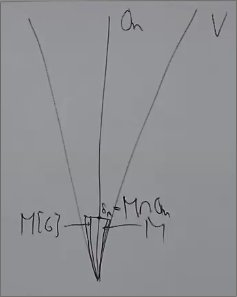
\includegraphics[width=0.5\textwidth]{MG}
  \caption{World of \(M[G]\) and \On}
  \label{fig:MG}
\end{figure}

Our goal if to have \(M[G]\) as a model of ZFC.

\begin{ldef} \label{def:unordered:pair}
Givne names \(\sigma,\tau\), we define \emph{unordered pair}
\(\up(\sigma,\tau) = \{(\sigma,0_\dsP),(\tau,0_\dsP)\}\).
\end{ldef}

\begin{claim}
For all names \(\sigma,\tau\), \(\{\sigma_G,\tau_G\}\).
\end{claim}

\begin{ldef} \label{def:ordered:pair}
Givne names \(\sigma,\tau\), we define \emph{ordered pair}
\(\op(\sigma,\tau) = \up(\up(\sigma, \sigma), \up(\sigma,\tau))\).
This is evaluated to \((\sigma_G,\tau_G)=\{\{\sigma_G\},\{\sigma_G,\tau_G\}\}\).
\end{ldef}

\begin{claim}
\(M[G] \models \textnormal{pairing axiom}\).
\end{claim}
\begin{proof}
Simple build of pair of names.
\end{proof}

\begin{claim}
\(M[G] \models \textnormal{infinity axiom}\).
\end{claim}
\begin{proof}
Simply by \(M\subseteq M[G]\).
\end{proof}

\begin{claim}
\(\forall a\in M[G]\, \exists b\in M[G]\, \cup a \subseteq b\).
\end{claim}
With separation we get the union axiom.
\begin{proof}
Let \(a\in M[G]\) be some set. We have a class of names \(\sigma\in M^\dsP\)
such that \(a = \sigma_G\).
Looking on first coordinate, \(\dom(\sigma)\) (set of names).
Take \(\up = \cup \dom(\sigma) \in M^\dsP\).
Put \(b=\pi_G\). We will show that \(\cup a \subseteq b\).
Let \(c\in \cup a\) we will show that \(c\subseteq b\).
From \(a\in c\) there exist \((\tau,p)\in \sigma\) and \(p\in G\).
such that \(c = \tau_G\). Therefore \(\tau \subseteq \cup \dom \sigma\)
and \(c = \tau_G \subseteq (\cup\dom\sigma)_G = \pi_G = b\).
\end{proof}

We still have some more complicated axioms.
This is going to be the essential subject of the course.
Using forcing technique.

%%%%%%%%%%%%%%%%%%%%%%%%%%%%%%%%%%%%%%%%%%%%%%%%%%%%%%%%%%%%%%%%%%%%%%%%
\subsection{Forcing --- 3 Lemmas}

\iffalse
\begin{ldef}
Let \(p\in\dsP\), \(\Phi\) a formula in the language of set theory.
\(p \Vdash \Phi\) ($p$ \emph{forces} \(\Phi\)) iff
for each generic \(G\subseteq \dsP\), \(p\in G\)
we have \(M[G] \models \Phi\).
\end{ldef}
\fi

\begin{ldef}
Let \(p\in\dsP\), \(\Phi(\seqn{v})\) a formula in the language of set theory,
\((\seqn{\sigma})\in M^\dsP\)
\(p \Vdash \Phi(\seqn{v})\) ($p$ \emph{forces} \(\Phi\)) iff
for each generic \(G\subseteq \dsP\), \(p\in G\)
we have \(M[G] \models \Phi(\sigma_{1G},\ldots,\sigma_{nG})\).
\end{ldef}

We present the following 3 lemmas.

% Lemma of definability.
\begin{lemma}[Definability]
Let \(\Phi(\seqn{v})\) be a formula, then
\begin{equation*}
\left\{(p,\seqn{\sigma})|\, p\in \dsP, \seqn{\sigma}\in M^\dsP,
  p\Vdash \Phi(\seqn{\sigma})\right\}
\end{equation*}
is a class in $M$.
\end{lemma}

A second
\begin{lemma}[The Extension]
If \(p\Vdash \Phi\) and \(p\leq q\) then \(q\Vdash \Phi\).
\end{lemma}

And last lemma (for now)
\begin{lemma}[The truth]
For each generic \(G\subseteq \dsP\)
\(M[G] \models \Phi\)
iff \(\exists p\in G\, p\Vdash \Phi\).
\end{lemma}
Note: \(\Phi\) can have variables.

In order to prove the 3 lemmas, we will define
a (\emph{weak forcing}) variant of \forcesstar\ of
\forces.
We will prove the 3 lemmas, replacing \forces\ by \forcesstar\
and show for each formula \(\Phi\) and each \(p\in\dsP\),
\(p\forces \Phi\) iff \(p \forcesstar \neg\neg\Phi\).
Then in the 3 lemmas we will replace \(\Phi\) by \(\neg\neg\Phi\).

%%%%%%%%%%%%%%%%%%%%%%%%%%%%%%%%%%%%%%%%%%%%%%%%%%%%%%%%%%%%%%%%%%%%%%%%
\subsection{Defining Weak Forcing --- \forcesstar}

In formulas we have connectors, quantifiers: \(\neq\), \(\lor\), \(\exists\)
and relations \(\in\) and \(\neq\). We can use \(\neg\neq\) for $=$.
We now define \forcesstar.

Let \(a,b\) names, \(p\in\dsP\). By inductive recursion in $M$
\begin{align}
p \forcesstar a\in b &\;\Leftrightarrow\; \exists c \exists q\leq p
 \land b\in(c,q) \land p \forcesstar a=c \label{eq:pforce:in} \\
p \forcesstar a \neq b &\;\Leftrightarrow\; \exists c \exists q\leq p
 \bigl( (c,q)\in a \land p\forcesstar c\notin b\bigr)
 \lor
 \bigl( (c,q)\in b \land p\forcesstar c\notin a\bigr) \label{eq:pforce:neq} \\
p \forcesstar \neg\Phi &\;\Leftrightarrow\;
 \forall p\leq q\, p\not\forcesstar\Phi \label{eq:pforce:neg} \\
p \forcesstar (\Phi \lor\Psi) &\;\Leftrightarrow\;
  p \forcesstar \Phi \lor p \forcesstar \Psi \label{eq:pforce:or} \\
p \forcesstar \exists v\,\Phi(v) &\;\Leftrightarrow\;
 \exists b \;\textnormal{(a name)} \, p \forcesstar \Phi(b).
   \label{eq:pforce:exists}
\end{align}

% lecture break

%%%%%%%%%%%%%%%%%%%%%%%%%%%%%%%%%%%%%%%%%%%%%%%%%%%%%%%%%%%%%%%%%%%%%%%%
\subsection{\forcesstar\ lemmas}

\begin{lemma}[\forcesstar-Extension]
If \(p \forcesstar \Phi\,\land\,p \leq q\) then \(q\forcesstar \Phi\).
\end{lemma}
\begin{proof}
Assume \(q\geq p \forcesstar \Phi\), we will show \(q\forcesstar \Phi\).
There is no \(r'\geq r\) such that \(r'\forcesstar \Phi\)
since \(r' \geq p\).
Therefore \(r' \not\forcesstar \Phi\). Thus \(r \forcesstar \neg \Phi\).

Justifying (\ref{eq:pforce:or}) and (\ref{eq:pforce:exists})
can be done by induction.
\end{proof}

\begin{lemma}[The truth \forcesstar]
For each generic \(G\subseteq \dsP\)
\(M[G] \models \Phi\)
iff \(\exists p\in G\, p\forcesstar \Phi\).
\end{lemma}
\begin{proof}
Let generic \(G\subseteq \dsP\). Assume \(M[G] \models a_G \in b_G\).
Then there exist a name $c$ and \(q\in G\) such that \((c,q)\in b\)
and \(M[G] \models a_G = c_G\). By induction \(\exists r\in G\)
such that \(r\forcesstar a=c\). Being generic, we have \(p\in G\)
such that \(q,r\leq p\) and then \(p\forcesstar a=c\).
Now by (\ref{eq:pforce:in}) \(p\forcesstar a\in b\).

Opposite direction. Assume \(p\in G\) and
 \(\exists c \exists q\leq p \land b\in(c,q) \land p \forcesstar a=c\).
From latter assumptions \(q\in G\), \(c_G\in b_G\) and \(a_G = c_G\).

Handling (\ref{eq:pforce:neq}) is similar, left as exercise.

Negation connector. Assume
 \(M[G] \models\neg\Phi\).
We have
 \(M[G] \models\neg\Phi \Leftrightarrow M[G] \not\models\Phi\).
Also \(\Leftrightarrow \neg(\exists q\in G\, q\forcesstar \Phi)\).
We need
\begin{claim}
The set \(D = \{r\in\dsP|\, r\forcesstar\Phi \lor r\forcesstar \neg\Phi\}\)
is dense (in $M$).
\end{claim}
\begin{proof}
Let \(t\in\dsP\). If \(\exists r\geq t\, r\forcesstar\Phi\) then \(r\in D\).
Otherwise, \(\forall r\geq t\, r \not\forcesstar \Phi\)
and then \(t\forcesstar\neg\Phi\).
\end{proof}
Back to the lemma. \(G\cap D\neq \Phi\),
therefore \(\exists p\in G\, p\forcesstar \neg\Phi\).

Conversely, assume \(\exists p\in G\, p\forcesstar \neg\Phi\)
and by negation \(M[G]\not\models\Phi\) and so \(M[G]\models\neg\Phi\).
By induction, \(\exists r\in G\, r\forcesstar\Phi\).
So \(\exists q\in G\,q\geq p,r\). By the \forcesstar-extension lemma,
\(q\forcesstar\Phi\) which contradicts (\ref{eq:pforce:neg}).

Showing the last two equivalences
(\ref{eq:pforce:or}) and (\ref{eq:pforce:exists}) are trivial.
\end{proof}

%%%%%%%%%%%%%%%%%%%%%%%%%%%%%%%%%%%%%%%%%%%%%%%%%%%%%%%%%%%%%%%%%%%%%%%%
\subsection{Connecting \forces\ with \forcesstar}.

\begin{claim}
For any \(p\in\dsP\) and any formula \(\Phi\),
\(p\forces\Phi\) iff \(p\forcesstar\,\neg\neg\Phi\).
\end{claim}
\begin{proof}
Assume \(p\forces \Phi\) and by negation \(p\not\forcesstar\neg\neg \Phi\).
Then \(\exists q\geq p\, q \forcesstar \neg\Phi\).
Let \(G\subseteq\dsP\) be generic such that \(q\in G\).
By the truth-\forcesstar lemma, \(M[G]\models \neg\Phi\) but \(q\geq p\)
implies \(p\in G\) contradiction to the \forces\ definition.

Conversely, let \(p\forces \neg\neg \Phi\).
By the truth-\forcesstar\ lemma, \(M[G]\models \neg\neg\Phi\),
then \(M[G]\models Phi\).
Since $G$ is arbitrary as long as \(p\in G\), hence \(p\forces \Phi\).
\end{proof}

%%%%%%%%%%%%%%%%%%%%%%%%%%%%%%%%%%%%%%%%%%%%%%%%%%%%%%%%%%%%%%%%%%%%%%%%
\subsection{Satisfying Separation axiom}

\begin{claim}
\(M[G]\models \textnormal{Separation axiom}\).
\end{claim}
\begin{proof}
Let a set \(S\in M[G]\) and a formula \(\phi(\seqn{v})\)
and \(\seqn{x}\in M[G]\).
We look at \(X=\{a\in A|\,M[G]\models \phi(\seqn{x})\).
% where \seqn{x} are names.
We need to show \(X\in M[G]\).
We need to build a name for it.
Pick \(\utilde{A}\) and
% \seqn{\utilde{x}}
\(\utilde{x}_1,\ldots,\utilde{x}_2\)
names such that \(A={\utilde{A}}_G\) and \(x_i={\utilde{x}_i}_G\).
Let
\begin{equation*}
X = \left\{((\utilde{a},p)\,|\, \utilde{a}\in\dom(\utilde{A})\,\wedge\,
  p\in\dsP \,\wedge\,
  p\forces(\utilde{a}\in\utilde{A}) \,\wedge\,
  p\forces \phi(\utilde{a},\utilde{x}_1,\ldots,\utilde{x}_n)
  \right\}.
\end{equation*}
We will show \(X=\utilde{X}_G\).

(\(\subseteq\):) Let \(a\in X\), then \(a\in A\) so there exists
\(\utilde{a}\in\dom(\utilde{A})\) such that \(a=\utilde{a}_G\).
Now \(M[G]\models a\in A\), \(M[G] \models \phi(a,\seqn{x})\).
and from the truth lemma there is (a stronger) \(p\in G\) such that
\begin{align}
p &\forces \utilde{a} \in \utilde{A} \label{eq:pforce:aA} \\
p &\forces \phi(\utilde{a},\utilde{x}_1,\ldots,\utilde{x}_n).
  \label{eq:pforce:phix}
\end{align}
We see that \((\utilde{a},p)\in \utilde{X}\).
Since $p$ in a generic set, \(a\in \utilde{X}_G\).

(\(\supseteq\):) Let \(\in \utilde{X}_G\).
Then \(\exists (\utilde{a},p)\in\utilde{X}\,
  (p\in G\,\land\,a={\utilde{a}}_G)\).
From \((\utilde{a},p)\in\utilde{X}\)
we have (\ref{eq:pforce:aA}) and (\ref{eq:pforce:phix}).
From \(p\in G\) we have \(M[G] \models \phi(a,\seqn{x})\)
and \(a\in X\) as desired.
\end{proof}

%%%%%%%%%%%%%%%%%%%%%%%%%%%%%%%%%%%%%%%%%%%%%%%%%%%%%%%%%%%%%%%%%%%%%%%%
%%%%%%%%%%%%%%%%%%%%%%%%%%%%%%%%%%%%%%%%%%%%%%%%%%%%%%%%%%%%%%%%%%%%%%%%
\section{2026/May/3}

Note: The first hour of the lecture lacked video recording.

%%%%%%%%%%%%%%%%%%%%%%%%%%%%%%%%%%%%%%%%%%%%%%%%%%%%%%%%%%%%%%%%%%%%%%%%
\subsection{Refresh}

We have forcing notion \lrangle{\dsP, \leq_\dsP, 0_\dsP},
partially ordered. A transitive countable model $M$.
We wish to build a gerneric extension.
\(G\subseteq\dsP\) is called generic iff
\begin{enumerate}[label={(\alph*)}]
\item \(\forall p,q\in\dsP\;((p\in G \land q\leq p) \implies q\in G)\).
\item \(p,q\in G\;\implies\; \exists r\in G (p,q\leq r)\).
\item For each dense \(D\subseteq \dsP\) \label{item:dense:DG}
  if \(D\in M\) then \(G\cap D\neq\emptyset\).
\end{enumerate}

\B{Note:} In requirement \ref{item:dense:DG} instead of dense $D$,
we can use maximal antichain (exercise).

\(M^\dsP\) is the class of names.
A name is a set consisting of pairs \((\sigma,p)\),
wher \(\sigma\) is a name and \(p\in\dsP\).
This is a recursive definition in the rang of \(\sigma\).

Given \(\tau\in M^\dsP\),
we have \(\tau_G = \{\sigma_G|\,\exists p\in G\, (\sigma,p)\in\tau\}\).

A generic extension: \(M[G] = \left\{\tau_G|\,\tau\in M^\dsP\right\}\).
We saw
\begin{enumerate}
\item \(M[G]\cap \On = \On\).
\item \(M[G]\) is a transitive model. For any model $N$ of
  set theory if \(M\subseteq Q\) and \(N\in G\) then \(M[G]\subseteq N\).
\item \(M[G]\) satisfied the extensionality, pairing, union, infinity,
  regularity and separation axioms.
\end{enumerate}

In order to show separation, we use
\begin{ldef}
\(p\forces \phi\) iff
\(\forall G \subseteq \dsP\, (p\in G \implies M[G]\models \phi)\).
\end{ldef}

We had extension and truth lemmas.
The latter says:
\(M[G] \models \phi\) iff \(\exists p\in G\, p\forces \phi\).

%%%%%%%%%%%%%%%%%%%%%%%%%%%%%%%%%%%%%%%%%%%%%%%%%%%%%%%%%%%%%%%%%%%%%%%%
\subsection{M[G] and Separation Axiom}

\begin{claim}
\(M[G]\) satisfies the replacement (scheme) axiom.
\end{claim}
\begin{proof}
Given a formula \(\phi(x)\) and a set \(A\in M[G]\).
Assume \(M[G]\models \forall a\in A\,\exists! y \phi(a,y)\).
We will show there exists \(B\in M[G]\) such that
\(\forall a\in A\,\exists b\in B\, M\models \phi(a,b)\).
Let \utilde{A} be a name of $A$, that is \(\utilde{A}_G = A\).
There exists $b$ such that \(M[G]\models \phi(a,b)\).
By the truth lemma there exists \(p \in G\) such that \(p\forces \phi(a, b)\).
We will work in (ground model?) $M$.
Define a function \(F:\dom \utilde{A}\times\dsP\to\On\).
Let \(F(\sigma,p)=\alpha\,\Leftrightarrow\)
\(\alpha\) is the smallest ordinal such that there exists a name \(\tau\)
such that \(p\forces \phi(\sigma,\tau)\).
If there does not exists such \(\alpha\) the we let \(F(\sigma,p)=0\).

Now we can bound. There exists \(\alpha^*\) such that
\(\forall (\sigma,p)\, F(\sigma,p)<\alpha^*\).
Let $S$ be the set of all names with rank \(<\alpha^*\).

{\small Note: At the point video recording started, non focused.}

Put \(\utilde{B} = S\times\{0_\dsP\}\).
We will show that \utilde{B} is as required.
We will show that
\(M[G]\models \forall a\in A\,\exists b\in B\,\phi(a,b)\)
where \(B=\utilde{B}_G\).
Look at \(F(\utilde{a},p)\) in the above case where \(\alpha\) exists.
We get \(F(\utilde{a},p)\leq \alpha^*\).
There exists \(\tau\in S\) such that \(p\models \phi(\utilde{a},\tau)\)
therefore \(M[G]\models \phi(a,\tau_G)\).
This shows the replacement axiom.
\end{proof}

%%%%%%%%%%%%%%%%%%%%%%%%%%%%%%%%%%%%%%%%%%%%%%%%%%%%%%%%%%%%%%%%%%%%%%%%
\subsection{M[G] and Power Axiom}

We now turn to the power axiom, which is the the problematic one to show.
We must be careful, when adding real since we may
add undesired subsets.

\begin{claim}
\(M[G]\) satisfies the power axiom.
\end{claim}
\begin{proof}
Let \(A\in M[G]\). We will show that
\begin{equation*}
\left(\Power(A)\right)^{M[G]} = \{a\in M[G]|\, a\subseteq A\} \in M[G].
\end{equation*}
The notation of left element in the above, means ``power within \(M[G]\)''.

We need to find a name. We will show that there exists \(B\in M[G]\)
such that for all \(a\subseteq A\) and \(a\in M[G]\)
implies \(a\subseteq B\). In $M$, let us look at
\begin{equation*}
\{\tau\in M^\dsP|\,\dom\tau \subseteq \dom \utilde{A}\}
  = \Power(\dom\utilde{A}\times\dsP)^M
\end{equation*}
Given a set $S$ of names, we want to convert it to a name:
\(\utilde{B} = S\times{0_\dsP}\).

Let \(x\subseteq A\), \(x\in M[G]\) and pick a name \(\utilde{x}\)
such that \(\utilde{x}_G = x\).
We will show that then
\(x\in B = \utilde{B}_G\).

{\small at the point the video is focused on board}

Define another name
\(\tau = \{(\tilde{a},p)|\,
  \utilde\in\dom\utilde{A}\,\land\,
  p\forces \tilde{a}\in\utilde{x}\}\).\\
Now
  \(\dom \tau \subseteq \dom\utilde{a}
    \;\implies \tau \in S
    \;\implies \tau_G \in \utilde{B}_G = B\).

\begin{subclaim}
\(\tau_G = x\).
\end{subclaim}
\begin{proof}
(\(\subseteq\)): Let \(y\in\tau_G\) so there exist \(p\in G\)
and \utilde{y} such that \((\utilde{y},p)\in\tau\) and \(\utilde{y}_G=y\).
Since \((\utilde{y},p)\in\tau\), we have \(p\forces y\in x\)
and by the truth lemma \(y\in x\).

(\(\supseteq\)): Let Let \(y\in x\subseteq A\) and \utilde{y} a name for it,
\(\utilde{y}_G = y\) such that \(utilde{y}\in\dom A\).
This can be found, since \(y\in A\).
\(y\in x\) implies \(\exists p\in G\, p\forces \utilde{y}\in\utilde{x}\).
Thus \((\utilde{y},p)\in\tau_G\), \(p\in G\)
and so \(y = \utilde{y}_G\in\tau_G\).
\end{proof}

This finshes the proof of the power axiom main claim.
\end{proof}

%%%%%%%%%%%%%%%%%%%%%%%%%%%%%%%%%%%%%%%%%%%%%%%%%%%%%%%%%%%%%%%%%%%%%%%%
\subsection{M[G] and Axiom of Choice}

The last axiom we want to show
\begin{claim}
\(M[G] \models \AC\).
\end{claim}
\begin{proof}
Let \(A\in M[G]\) and \utilde{A} a name for it.
$M$ satisfies \AC\ so it has a partial order. Using it
we look at
\(\dom\utilde{A} = \{\pi_\gamma|\,\gamma\in\delta\}\).

Refreshing \ref{def:unordered:pair} and \ref{def:unordered:pair}
\begin{align*}
\up(\sigma,\tau) &= \{(\sigma,0_\dsP),(\tau,0_\dsP)\} \\
(\up(\sigma,\tau))_G &= \{\sigma_G,\tau_G\} \\
\op(\sigma,\tau) &= \{(\up(\sigma,\sigma),0_\dsP), \up(\sigma,\tau),0_\dsP),
\end{align*}
we define
\begin{equation*}
S = \{\op(\breve{\gamma},\pi_\gamma)|\,\gamma<\delta\}
\end{equation*}
where \(\breve{\gamma}\) is a canonical name for \(\gamma\).
We want to make the set $S$ of names to a name
\begin{equation*}
(S\times\{0_\dsP\})_G = \{(\gamma,\pi_\gamma)|\, \gamma<\delta\}
\end{equation*}
Containing
\begin{equation*}
\{(\pi_\gamma)_G|\,\gamma<\delta\} \subseteq A
\end{equation*}
on which we have a well order. Thus \AC.
\end{proof}

With this, we completed showing the generic extension is a model for \ZFC.

%%%%%%%%%%%%%%%%%%%%%%%%%%%%%%%%%%%%%%%%%%%%%%%%%%%%%%%%%%%%%%%%%%%%%%%%
\subsection{Cohen-Real Forcing}

Let
\begin{equation*}
C = \left\{p|\, p\;\textnormal{partial finite function}: \omega\to 2\right\}.
\end{equation*}
With the continuation order \(q\leq p\;\Leftrightarrow q \subseteq p\).
Let \(G\subseteq C\) be generic. Let \(g=\cup G\)
which is a function, since being generic, there no inconsistencies in $G$.
We alreadt saw that \(g:\omega \to 2\) is a complete function
and \(g\notin M\).
For any \(h\in M\), look at
\(D^j = \{p\in C|\, \exists n\in\dom p\, p(n)\neq h(n)\}\).
which is dense. Thus \(G\cap D^h\neq\emptyset\) and so \(g\neq h\).

\B{Conclusion}: \(V \neq L\) (G\"odel model) is consistent.
or
\begin{equation*}
M[G] \models \textnormal{There exists real not constructible, not in }L.
\end{equation*}

Let \(\lambda\) be a cardinal and
\begin{equation*}
C(\lambda) =
  \left\{p|\, p\;\textnormal{partial finite function}:
    \omega\times\lambda\to 2\right\}.
\end{equation*}
Here we try to build Cohen-\(\lambda\)-real forcing.
Let \(G\subseteq C(\lambda)\) be generic. For each \(\alpha<\lambda\)
define \(g_\alpha:\omega\to 2\) by
\(g_\alpha(n) = (\cup G)(n,\alpha)\).
\begin{enumerate}[label={(\alph*)}]
\item \(\forall \alpha<\gamma\, g_\alpha\notin M\).
\item \(\forall \alpha,\beta<\gamma\,
  (\alpha\neq\beta\,\implies\,g_\alpha\neq g_\beta)\).
\end{enumerate}

If we take \(\lambda=\aleph_2\) we get \(\aleph_2\) different functions.
This ``almost'' contradicts \CH.
So far we have not disussed cardinals. Being cardinal,
is not necessarily maintained in other model(?).

%%%%%%%%%%%%%%%%%%%%%%%%%%%%%%%%%%%%%%%%%%%%%%%%%%%%%%%%%%%%%%%%%%%%%%%%
\subsection{Cardinals in M[G]}

\begin{ldef}
\begin{enumerate}[label={(\alph*)}]
\item \(M[G]\) \emph{preserves cardinalities} iff for each cardinal
  \(\kappa\) in $M$, \(\kappa\) is still a cardinal in \(M[G]\).
  Note: the converse is trivial. \(M[G]\) has more functions,
  it is ``harder '' to be a cardinal there.
\item \(M[G]\) \emph{preserves cofinality} iff for each cardinal
  \(\kappa\) in $M$
  \begin{equation*}
    (\cof(\kappa))^M = (\cof(\kappa))^{M[G]}.
  \end{equation*}
\item \(M[G]\) \emph{preserves regularity}
  If every regular cardinal in $M$ remains like this in \(M[G]\).
\end{enumerate}
\end{ldef}

\begin{claim}
If \(M[G]\) preserves cofinality, then \(M[G]\) preserves cardinalities.
\end{claim}
\begin{proof}
By negation, assumes \(M[G]\) does not preserves cardinalities.
Let \(\kappa\) be the smallest cardinal in $M$
that is not a cardinal in \(M[G]\).
Clealy \(\kappa\) cannot be neither finite nor \(\omega\).
Since it is the firsr, it also cannot be a limit cardinal.
By looking at preceding functions, see figure \ref{fig:non-lim-kappa}.
\begin{figure}[H]
  \centering
  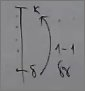
\includegraphics[height=0.2\textheight]{kappa-non-limit}
  \caption{Non limit \(\kappa\)}
  \label{fig:non-lim-kappa}
\end{figure}
Thus \(\kappa\) is a successor cardinal, and so it is regular cardinal in $M$.
But \(\kappa\) is not a cardinal in \(M[G]\) so it cannot be regular.
A contradiction.
\end{proof}
Note that here we did not use generic $G$.

\begin{claim}
If \(M[G]\) preserves regularity then it preserves cofinality.
\end{claim}
\begin{proof}
By negation, there exists a limit order \(\delta\) such that
\begin{equation*}
  \rho = (\cof(\delta))^M \neq (\cof(\kappa))^{M[G]} = \mu.
\end{equation*}
Then \(\rho > \mu\). Then we have two one-to-one unbounded functions:
\begin{align*}
 f_\rho&: \rho \to \delta \\
 f_\mu&: \mu \to \delta
\end{align*}
Then we can build a one-to-one unbounded \(f:\mu\to\rho\)
(see figure \ref{fig:mulambdarow})
\begin{figure}[H]
  \centering
  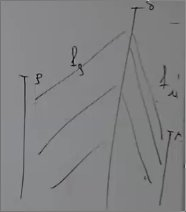
\includegraphics[height=0.4\textheight]{rho-lambda-mu}
  \caption{\(\rho\rightarrow\lambda\leftarrow\mu\)}
  \label{fig:mulambdarow}
\end{figure}
Thus \(\rho\) changed it cofinality in \(M[G]\) to \(\mu\),
a contradiction.
\end{proof}
Again we (did not need?) generic extension(?).

%%%%%%%%%%%%%%%%%%%%%%%%%%%%%%%%%%%%%%%%%%%%%%%%%%%%%%%%%%%%%%%%%%%%%%%%
\subsection{Countable Chain Condition}

\begin{ldef}
\lrangle{\dsP,\leq_\dsP,0_\dsP} in $M$ satisfies
\emph{countable chain condition} (\ccc) iff
for any chain \(A\subseteq \dsP\), \(|A|\leq\aleph_0\).
\end{ldef}
Clearly if \(|\dsP|=\aleph_0\) then \dsP\ satisfies \ccc.

\begin{claim}
Let \(G\subseteq\dsP\) be generic, and \dsP satisfies \ccc.
Assume there exist \(\alpha,\beta\) ordinals
and a function \(f:\alpha\to\beta\) in \(M[G]\).
Then there exists a function \(F:\alpha\to\Power(\beta)\) in $M$
such that for all \(\gamma<\alpha\)
\begin{enumerate}
\item \(f(\gamma)\in F(\gamma)\). \label{item:f:gamma:F}
\item \(|F(\gamma)|\leq\aleph_0\). \label{item:f:gamma:aleph0}
\end{enumerate}
\begin{figure}[H]
  \centering
  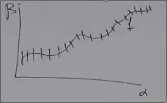
\includegraphics[height=0.2\textwidth]{func-alphabeta-cover}
  \caption{Cover of \(f:\alpha\to\beta\)}
  \label{fig:func:alphabeta:cover}
\end{figure}
\end{claim}
Intuitively, we want to have a delicate cover of $f$ by $F$ in the old model.
\begin{proof}
Let \(f:\alpha\to\beta\) in \(M[G]\). Then there exists \(p\in G\)
and a name \utilde{f} of $f$ such that
 \(p \forces \utilde{f}:\breve{\alpha}\to\breve{\beta}\)
(canonical names).

We will work in $M$. Define
\begin{equation*}
F(\gamma) = \{\delta<\beta|\,\exists q\geq p\, q\forces
  \utilde{f}(\breve{\gamma})=\breve{\delta}\}.
\end{equation*}
We need to check the two requirements above.

Checking \ref{item:f:gamma:F}.
Let \(\gamma<\alpha\). There exists \(\beta>\delta\) such that
\(f(\gamma)=\delta\) in \(M[G]\).
By the truth lemma, there exists \(q\geq p\), \(q\in G\) such that
\(q\forces \utilde{f}(\breve{\gamma})=\breve{\delta}\).
Then \(\delta\in F(\gamma)\).

Checking \ref{item:f:gamma:aleph0}.
In $M$, assume that, \(\delta_1,\delta_2\in F(\gamma)\)
and \(\delta_1\neq\delta_2\) and \(\gamma<\alpha\).
Then we have \(q_i \forces \utilde{f}(\breve{\gamma})=\breve{\delta}_i\)
for \(i=1,2\).
We need to show that \(q_1,q_2\) are not compatible.
By negation, \(\exists r\geq p\leq q_1,q_2 \geq p\).
Now
\begin{align}
p & \forces \utilde{f}: \breve{\alpha} \to \breve{\beta} \nonumber \\
r & \forces \utilde{f} \; \textnormal{is a function} \nonumber \\
r & \forces \utilde{f}(\breve{\gamma}) = \breve{\delta}_i
    \quad \textnormal{for both}\; i=1,2 \label{eq:force:delta12}
\end{align}
Note that \eqref{eq:force:delta12} is not an immediate contradiction.

If \(r\in G\) then we could have picked. But we do not assume this.

Let \(H\subseteq \dsP\) be generic such that \(r\in H\).
In \(M[H]\), we look at \(g = \utilde{g}_H\).
\begin{equation*}
 M[H] \models g: \alpha\to \beta \quad \textnormal{is a function}.
\end{equation*}
The canonical names \(\breve{\alpha}\), \(\breve{\beta}\)
are always the same, no matter what generic is used.
Applying to \eqref{eq:force:delta12}, we get the contradiction
\begin{equation*}
g(\gamma) = \delta_1 \neq \delta_2 = g(\gamma).
\end{equation*}
\end{proof}

%%%%%%%%%%%%%%%%%%%%%%%%%%%%%%%%%%%%%%%%%%%%%%%%%%%%%%%%%%%%%%%%%%%%%%%%
%%%%%%%%%%%%%%%%%%%%%%%%%%%%%%%%%%%%%%%%%%%%%%%%%%%%%%%%%%%%%%%%%%%%%%%%
\section{2026/May/10}

%%%%%%%%%%%%%%%%%%%%%%%%%%%%%%%%%%%%%%%%%%%%%%%%%%%%%%%%%%%%%%%%%%%%%%%%
\subsection{Refresh}

We have a model $M$, \(\lrangle{\dsP, \leq_\dsP, 0_\dsP} \subseteq M\),
a generic \(G\subseteq \dsP\) and (class?) of names \(M^\dsP \subseteq M\).
\begin{center}
\begin{tabular}{ll}
$M$ & \(M[G]\) \\
Ground model & Generic extension \\
\multicolumn{2}{c}{\ZFC} \\
\multicolumn{2}{c}{\(M\cap\On = \On\)}
\end{tabular}
\end{center}

We had the truth lemma saying:
\begin{equation*}
M[G]\models\phi\;\Leftrightarrow\; \exists p\in G\,p\forces \phi.
\end{equation*}

What about cardinals? \\
$M$ and \(M[G]\) agree about cardinals till \(\aleph_0\).
if \(\kappa\) is a cardinal in \(M[G]\) then it is a cardinal in $M$
because \(M\subseteq M[G]\).

\begin{enumerate}[label={(\alph*)}]
\item Preserve cardinalities. \label{item:pres:card}
\item Preserve cofinality. \label{item:pres:cof}
\item Preserve regular cardinals. \label{item:pres:regcard}
\end{enumerate}

We have
\begin{equation*}
 \textnormal{\ref{item:pres:card}}
 % \;\overset{\Longleftarrow}{\not\Longrightarrow}\;
 \;\mathrel{\substack{\Longleftarrow \\ \centernot\Longrightarrow}}\;
 \textnormal{\ref{item:pres:cof}}
 \;\Longleftrightarrow\;
 \textnormal{\ref{item:pres:regcard}}
\end{equation*}

\ccc\ in $M$ --- For each anti-chain \(A\subseteq\dsP\), \(|A|\leq\aleph_0\).
By \ccc\ we mean
 \(\forall p,q\in A\, (p\neq q \implies \not\exists r\, p,q\leq r)\).

\begin{claim}
Assume \dsP\ satisfies \ccc. Let \(G\subseteq\dsP\) generic.
Assume in \(f:\alpha\to\beta\) in \(M[G]\) then in $M$ there exists
\(F:\alpha\to\Power(\beta)\) such that for all \(\gamma<\alpha\)
\(f(\alpha)\in F(\alpha)\subseteq\beta\)
and the cardinality in $M$ of \(F(\alpha)\) is finite or countable.
\end{claim}

Let \(\gamma\) and arbitrary ordinal. Let Cohen focring
\begin{equation*}
C(\gamma) = \{f|\, f:\gamma\times\omega\to 2\; \textnormal{partial final}\}.
\end{equation*}
and \(G\subseteq C(\gamma)\) generic.
Define \(g_\alpha:\omega\to2\) by
\begin{equation*}
g_\alpha(n) = \left(\cup G\right)(\alpha,n).
\end{equation*}
For each \(\alpha,\beta<\gamma\), \(\alpha\neq\beta\)
we have \(g_\alpha\neq g_\beta\).

For each \(h\in M\), \(h:\omega\to2\) and for each \(\alpha<\gamma\),
\(h\neq g_\alpha\).
Thus in \(M[G]\) there exist at least \(\gamma\) functions \(\omega\to 2\).

%%%%%%%%%%%%%%%%%%%%%%%%%%%%%%%%%%%%%%%%%%%%%%%%%%%%%%%%%%%%%%%%%%%%%%%%
\subsection{Preservations}

\begin{claim}
Assume \dsP\ satisfies \ccc. Let \(G\subseteq\dsP\) be generic.
Then $M$ and \(M[G]\) have the same regular cardinals.
Therefore preserving cardinalities and preserving cofinalities are satisfied.
\end{claim}
\begin{proof}
Let \(\kappa\) be a regular cardinal of $M$. Assume \(\kappa>\aleph_0\).
Moving to \(M[G]\), let \(f:\delta\to\kappa>\) for \(\delta<\kappa\).
There exists \(F\in M\) such that \(\dom F=\delta\)
and for each \(\alpha<\delta\), \(|F(\alpha)|^M\leq\aleph_0\),
\(F(\alpha)\in F(\alpha)\). Define \(F^*:\delta\to\kappa\)
by \(\kappa > F^*(\alpha)=\sup F(\alpha)\).
For all \(\alpha<\delta\), \(f(\alpha)\leq F^*(\alpha\).
\(F^*\) is bounded in \(\kappa\) hence so is $f$.
\end{proof}

\begin{claim}
\(C(\lambda)\) satisfies \ccc\ for each \(\lambda\).
\end{claim}
Note: If \(\lambda<\aleph_0\) then any anti-chain \(\leq\aleph_0\).
\begin{proof}
Let \(\{f_i|\, i <\aleph_1\} \subseteq C(\lambda)\).
We will show that there exists \(S\subseteq \aleph_1\) such that
for all \(i,j\in S\), \(f_i\), \(f_j\) are compatible.
Denote \(a_i = \dom f_i\). We have \(\aleph_1\) finite subsets of
\(\lambda\times\omega\).
Then by \(\Delta\)-system,
there exists \(S\subseteq \aleph_1\),
\(|S|=\aleph_1\) and there exists \(a\leq\lambda\) finite
such that \(\forall i,j\in S\, (i\neq j\implies a_i\cap a_j=a)\).

How many functions \(a\to 2\) are there? \(2^{|a|}\).
Therefore there exists \(S^*\subseteq S\), \(|S^*|=\aleph_1\)
and there exists \(f:a\to 2\) such that for each \(i\in S^*\),
\(f{\restriction}_a = f\).

Pick \(i,j\in S^*\) and look at \(f_i\), \(f_j\).
If \(\dom f_i \cap \dom f_j \neq\emptyset\)
 pick \((\alpha,n)\in \dom f_i \cap \dom f_j = a_i\cap a_j\).
Now \(f_i(\alpha,n) = f(\alpha,n) = f_j(\alpha,n)\).
\end{proof}
Conclusion: We can break \GCH\ with \(\lambda\geq\aleph_?\).

%%%%%%%%%%%%%%%%%%%%%%%%%%%%%%%%%%%%%%%%%%%%%%%%%%%%%%%%%%%%%%%%%%%%%%%%
\subsection{Strengthening \ccc}

\begin{claim}
Let \(\lambda\) be regular cardinal \(>\aleph_0\).
Assume \(\{f_i|\, i < \lambda\} \subseteq C(\lambda)\).
Then there exists a stationary \(S\subseteq \lambda\)
such that for all \(i,j\in S\), \(f_i,f_j\) are compatible.
\end{claim}
This is stronger than \ccc.
\begin{proof}
Put \(a_i = \dom(\dom f_i)\) (taking first coordinate).
We have finite subsets \(\{a_i|\,i<\lambda\}\subseteq\lambda\).
Applying \(\Delta\)-system we have \(S\subseteq \lambda\)
and a finite \(a\subseteq\lambda\) such that for all \(i,j\in S\),
\((i\neq j\implies a_i\cap a_j = a\).
Look at the mapping \(i\to f_i{\restriction}_{a\times\omega}\)
the exist a stationary \(S^*\subseteq S\) and
a partial finite \(f:a\times\omega\to 2\) such that for all
\(i\in S^*\), \(f = f{\restriction}_{a\times\omega}\) and then for all
\(i,j\in S^*\) are compatible.
\end{proof}

%%%%%%%%%%%%%%%%%%%%%%%%%%%%%%%%%%%%%%%%%%%%%%%%%%%%%%%%%%%%%%%%%%%%%%%%
\subsection{Contradiction to \CH\ via \(\lambda\)}

\begin{thm}
Let \(\lambda>0\) be some ordinal. Let \(G\subseteq C(\lambda)\) be generic.
Then in \(M[G]\) there are at least \(\lambda\)
distinct functions \(\omega\to 2\).
Moreover, if \(\lambda\) is a cardinal \(\geq \aleph_2\) in $M$,
then it remains so also in \(M[G]\) and therefore
\(\aleph_2 \leq \lambda \leq 2^{\aleph_0}\) in \(M[g]\).
\end{thm}

\begin{corollary}
Let \(G\subseteq C(\aleph_2\) be generic. \(\aleph_2\) of $M$.
Then in \(M[G]\) \(\aleph_2\leq 2^{\aleph_0}\).
\end{corollary}

Question: Can we get equality?

%%%%%%%%%%%%%%%%%%%%%%%%%%%%%%%%%%%%%%%%%%%%%%%%%%%%%%%%%%%%%%%%%%%%%%%%
\subsection{Good Names Restriction}

Say we have \(X\subseteq\omega\). In \(M[G]\) there is a name \utilde{X}
such that \(X=\utilde{X}_G\), we have a mapping \(\utilde{X}\to\utilde{X}_G\).

We will try to get some bound.
We try to restrict the names.

\begin{ldef}
Let \(\delta\) be an arbitrary ordinal.
A name \(\tilde{a}\) is called a \emph{nice name} of subset of \(\delta\)
iff 
\(\utilde{a} = \bigl\{\{\breve{\alpha}\}\times A_\alpha|\, \alpha<\delta\bigr\}\)
where \(A_\alpha\subseteq \dsP\) is anti-chain.
\end{ldef}

\begin{claim}
Let $b$ be an arbitrary name such that 
\(0_\dsP\forces\utilde{b}\subseteq\breve{\delta}\).
Then there exist a nice name \utilde{a} such that
\(0_\dsP \forces \utilde{a} = \utilde{b}\).
\end{claim}

\begin{proof}
For each \(\alpha<\delta\) let \(A_\alpha\subseteq\dsP\) be anti-chain
such that 
\begin{enumerate}[label={(\alph*)}]
\item For each \(p\in A_\alpha\), \(p\forces \breve{\alpha} \in \utilde{b}\).
\item For each \(q\in\dsP\) if \(q\forces \breve{\alpha}\in\utilde{b}\)
  then there exists \(p\in A_\alpha\) such that $p$,$q$ are compatible.
\end{enumerate}

We will show that \(0_\dsP\forces \utilde{a}=\utilde{b}\).
Let \(G\subseteq\dsP\) generic. We will show \(a=\utilde{a}_G=\utilde{b}_G=g\).

(\(\subseteq\):). Let \(\alpha\in a\). We have \(\alpha=\breve{\alpha}_G\)
and \(a=\utilde{a}_G\) and there exists \(p\in A_\alpha\) and \(p\in G\)
The last two memberships respectable implies
\(p\forces \breve{a}\subseteq \utilde{b}\) and \(\alpha\in b\).

(\(\supseteq\):). Let \(\alpha\in b\).
There exists \(p\in G\), \(p\forces \breve{\alpha}\in b\).
If \(p\in A_\alpha\) then simply ... ?\\
If \(G\cap A_\alpha \neq \emptyset\) then \(q\in G\cap A_\alpha\)
and there exists \((\breve{\alpha},q) \in\utilde{a}\)
and so \(\alpha\in a\).

By negation, assume \(G\cap A_\alpha=\emptyset\),
then \(p\notin A_\alpha\).
Let
\begin{equation*}
D = \{r\in\dsP|\,
  (\exists q\in A_\alpha \land q<r) \lor
    (r\forces \breve{\alpha} \notin \utilde{b})
  \}.
\end{equation*}
We will show that $D$ is dense.
Let \(t\in\dsP\). If there exists \(r\geq t\) such that
\(r\forces \breve{\alpha}\notin\utilde{b}\) then \(r\in D\).
Assume there is no strengthening of $t$ that forces
\(\breve{\alpha}\notin\utilde{b}\), so thee exists \(r\geq t\) such that
\(r\forces \breve{\alpha}\in\utilde{b}\). If \(r\in A_\alpha\)
then we are done. Otherwise, there exists \(q\in A_\alpha\) that is compatible
with $r$, and let \(s\geq r,q\), \(s\in D\).
\end{proof}



%%%%%%%%%%%%%%%%%%%%%%%%%%%%%%%%%%%%%%%%%%%%%%%%%%%%%%%%%%%%%%%%%%%%%%%%
\subsection{Upper Bound on Power set}

\begin{claim}
Let \dsP\ be a forcing notion. Assum \(|\dsP|=\kappa\), \dsP\ satisfies
\ccc, \(\lambda\geq \aleph_0\). Let \(\theta = \kappa^\lambda\).
(So for in ground model). Let \(G\subseteq\dsP\) be generic.
Then \(2^\lambda\leq \theta\) in \MG.
\end{claim}
\begin{proof}
Compute amount of nice names of subsets of \(\lambda\).
\(\utilde{a} = \{\{\breve{\alpha}\}\times A_\alpha|\, \alpha<\lambda\}\)
where \(A_\alpha\) is anti-chain.
There are \(\kappa^{\aleph_0}\) anti-chains in \dsP.
For every \(\alpha<\lambda\) we choose an anti-chain \(A_\alpha\).
So all functions \(\lambda\to\) anti-chain, so their amount is
\(\left(\kappa^{\aleph_0}\right)^\lambda = \kappa^\lambda = \theta\)
the number of nice names.
\end{proof}

\begin{corollary}
Assume $M$ satisfies \GCH. Let \(G\subseteq C(\aleph_2)\) be a generic.
Then in \MG, \(2^{\aleph_0} = \aleph_2\).
And for all \(\alpha>0\), \(2^{\aleph_\alpha}=\aleph_{\alpha+1}\).
\end{corollary}
Thus in generic extension, we broke \GCH\ just in a single cardinal.

%%%%%%%%%%%%%%%%%%%%%%%%%%%%%%%%%%%%%%%%%%%%%%%%%%%%%%%%%%%%%%%%%%%%%%%%
\subsection{Exponents in \MG}

\B{Example}: Assume \(M\models\GCH\), \(G\subseteq C(\aleph_\omega)\).
We will compute exponents in \MG.
We have \(2^{\aleph_0} \geq \aleph_\omega\) since we added \(\aleph_\omega\)
distinct \(\omega\to 2\) functions.
From previous claim we have
\begin{align}
  2^{\aleph_0} &\leq \left({\aleph_\omega}^{\aleph_0}\right)^M \nonumber \\
&= \aleph_{\omega+1} \label{eq:aleph:omega+1}
\end{align}
The \eqref{eq:aleph:omega+1} equality holds since $M$ is a model of \GCH.
By K\"onig theorem \(2^{\aleph_0} \neq \aleph_\omega\),
so in this model \(2^{\aleph_0} = \aleph_{\omega+1}\).

\begin{itemize}
\item Assume \(\aleph_0\leq \label < \aleph_\omega\). Then
  \begin{equation*}
  \aleph_{\omega+1}
  = \left({\aleph_\omega}^\lambda\right)^M \geq 2^\lambda \geq \aleph_\omega.
  \end{equation*}
\item Assume \(\lambda \geq \aleph_\omega\).
  \begin{equation*}
  \lambda^+
  = \left({\aleph_\omega}^\lambda\right)^M \geq 2^\lambda \geq \lambda^+.
  \end{equation*}
  Therefore \(2^\lambda = \lambda^+\).
\end{itemize}

\begin{corollary}
Assume \(M\models\GCH\).
For all cardinal \(\lambda > \aleph_0\) such that \(\cof(\lambda)\neq\omega\)
in \(C(\lambda)\), \(2^{\aleph_0} = \lambda\).
\end{corollary}
\begin{proof}
Let \(G\subseteq C(\lambda)\) be generic.
\begin{equation*}
\lambda = \left(\lambda^{\aleph_0}\right)^M \geq 2^{\aleph_0} \geq \lambda
\end{equation*}
and therefore an equality.
\end{proof}

\begin{corollary}
Assume \(M\models\GCH\). Let \(\lambda\) be
strongly inaccessible cardinal
(regular and \(\forall \mu>\lambda, 2^\mu < \lambda\)).
Let \(G\subseteq C(\lambda)\) be generic.
Then in \MG\ is weakly inaccessible (regular and limit) but not strongly.
\end{corollary}

%%%%%%%%%%%%%%%%%%%%%%%%%%%%%%%%%%%%%%%%%%%%%%%%%%%%%%%%%%%%%%%%%%%%%%%%
\subsection{Uncountable Cardinals}

\begin{enumerate}[label={(\alph*)}]
\item How to get a state like
   \(2^{\aleph_0}=\aleph_1\;\land\;2^{\aleph_1}=\aleph_3\).
   That is \GCH\ breaks first in \(\aleph_1\) and not in \(\aleph_0\).
\item How to get a state like where \((\aleph_1)^M\) is countable in \MG.
\end{enumerate}

%%%%%%%%%%%%%%%%%%%%%%%%%%%%%%%%%%%%%%%%%%%%%%%%%%%%%%%%%%%%%%%%%%%%%%%%
\B{Collapse of \(\aleph_1\) (or \(\kappa\geq\aleph_1\))}

Let \(\kappa \geq\aleph_1\) be a cardinal. Let
\begin{gather*}
\Col(\aleph_0,\kappa) = \{f|\, f:\aleph_0\to\kappa \;\textnormal{final}\} \\
f_1 \leq f2 \;\Leftrightarrow\; f_1 \subseteq f_2.
\end{gather*}
This does not satisfy \ccc. Take \(\{\{(0,\alpha)\}|\,\alpha<\kappa\}\)
(partial functions mapping \(0\to\alpha\)),
an anti-chain of \(\kappa\) cardinality.
Take generic \(G\subseteq\Col(\omega,\kappa)\).
Then \(g=\cup G:\omega \xrightarrow{\text{onto}} \kappa\).
Therefore in \MG\ \(\kappa\) is countable.

\begin{ldef}
Let \(\kappa\) be a regular cardinal. \dsP\ \emph{satisfies \kcc}
iff for any anti-chain \(A\subseteq\dsP\), \(|A|\leq\kappa\).
\end{ldef}
Then \ccc\ \(\Leftrightarrow\) \(\kappa\)-c.c.

\begin{claim}
Assume \(\kappa\) is a regular cardinal. \dsP\ a forcing notion
that satisfies \kcc. Let \(G\subseteq \dsP\) be generic.
Assume in \MG\ \(f:\alpha\to\beta\).
Then in $M$ there exists a function $F$ from \(\alpha\) to \(\Power(\beta)\)
such that for eall \(\gamma<\alpha\) the following hold:
\begin{enumerate}
\item \(|F(\gamma) < \kappa\).
\item \(f(\gamma) \in F(\gamma)\).
\end{enumerate}
\end{claim}
Similar to what we had with \ccc, with similar proof.

\begin{claim}
Assume \dsP\ satisfies \kcc. Let \(G\subseteq\dsP\) be generic.
Then in \MG\ all the cardinals \(\geq\kappa\) are preserved.
\end{claim}
Similar proof as before. It is sufficient to look at successor cardinals.
\begin{figure}[H]
  \centering
  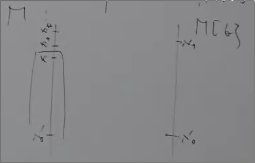
\includegraphics[width=0.4\textwidth]{MG-cardinals}
  \caption{Cardinals in $M$ and \MG}
  \label{fig:MG-cardinals}
\end{figure}

%%%%%%%%%%%%%%%%%%%%%%%%%%%%%%%%%%%%%%%%%%%%%%%%%%%%%%%%%%%%%%%%%%%%%%%%
%%%%%%%%%%%%%%%%%%%%%%%%%%%%%%%%%%%%%%%%%%%%%%%%%%%%%%%%%%%%%%%%%%%%%%%%
\section{2026/May/17}

%%%%%%%%%%%%%%%%%%%%%%%%%%%%%%%%%%%%%%%%%%%%%%%%%%%%%%%%%%%%%%%%%%%%%%%%
\subsection{Refresh}

We have shown that \(2^{\aleph_0} = \aleph_\alpha\) for all \(\alpha\)
such that \(\cof(\aleph_\alpha)>\aleph_0\).

\begin{ldef}
Given forcing notion \dsP, it is \kcc\ iff
for all anti-chain \(A\subseteq\dsP\), \(|A|<\kappa\).
\end{ldef}

\begin{claim}
Assume \dsP\ satisfies \kcc, \(G\subseteq\dsP\) generic, and a function
\(f:\alpha\to\beta\) in \MG\ then there exists a function \(F\in M\)
such that
\begin{enumerate}[label={(\alph*)}]
  \item \(\dom F = \alpha\).
  \item For eall \(\gamma<\alpha\)
    \begin{enumerate}[label={(\alph{enumi}\arabic*)}]
      \item \(F(\gamma)\subseteq \beta\).
      \item \(|F(\gamma)|<\kappa\).
      \item \(f(\gamma)\in F(\gamma)\).
    \end{enumerate}
\end{enumerate}
\end{claim}

\begin{claim}
Assume \dsP\ satisfies \kcc. Then fir each cardinals \(lambda\geq\kappa\), 
\(\kappa\) remains a cardinal in a generic extension.
\end{claim}

%%%%%%%%%%%%%%%%%%%%%%%%%%%%%%%%%%%%%%%%%%%%%%%%%%%%%%%%%%%%%%%%%%%%%%%%
\subsection{Generalization to Cardinals \(>\aleph_0\)}

Let \(\rho\), \(\mu\) be cardinals. Define
\begin{equation*}
\Cohen(\rho, \mu) = \{f|\, f:\mu\times\rho\to 2\;\land\;|f|<\rho\;
  \textnormal{partial}\},
\end{equation*}
With containing order: \(f_1\leq f_2\l\Leftrightarrow\;f_1\subseteq f_2\).
Take generic \(G\subseteq\Cohen(\rho, \mu)\) and
\(g = \cup G:\mu\times\rho\to 2\) and split for each \(\alpha<\mu\)
\(g_\alpha:\rho\to 2\) by \(g_\alpha(\beta) = g(\alpha,\beta)\).
We get \(\mu\) new and distinct functions \(\{g_\alpha|\, \alpha<\mu\}\).
In \MG\ we have \(|\Power(\rho)| \geq |\mu|\).

%%%%%%%%%%%%%%%%%%%%%%%%%%%%%%%%%%%%%%%%%%%%%%%%%%%%%%%%%%%%%%%%%%%%%%%%
%%%%%%%%%%%%%%%%%%%%%%%%%%%%%%%%%%%%%%%%%%%%%%%%%%%%%%%%%%%%%%%%%%%%%%%%
%%%%%%%%%%%%%%%%%%%%%%%%%%%%%%%%%%%%%%%%%%%%%%%%%%%%%%%%%%%%%%%%%%%%%%%%
\end{document}
